\documentclass{amsart}

\usepackage[T1]{fontenc}
\usepackage[utf8]{inputenc}
\usepackage[UKenglish]{babel}
\usepackage{amsmath}
\usepackage{amsthm}
\usepackage{amssymb}
\usepackage{float}
\usepackage{graphicx}
\usepackage{algorithm}
\usepackage{algorithmic}
\usepackage{todonotes}
\usepackage{enumitem}
\usepackage[misc]{ifsym}
\usepackage[foot]{amsaddr}
\usepackage[hidelinks]{hyperref}
\usepackage{csquotes}
\usepackage[style=authoryear,ibidtracker=false,uniquename=false,giveninits=true,terseinits=true,maxbibnames=5,backend=biber]{biblatex}
\renewbibmacro{in:}{}
\addbibresource{rnni_convexity.bib}

\newcommand{\np}{\mathcal{NP}}
\newcommand{\parent}{\mathrm{parent}}
\newcommand{\mrca}{\mathrm{mrca}}
\newcommand{\rank}{\mathrm{rank}}
\newcommand{\nni}{\mathrm{NNI}}
\newcommand{\rnni}{\mathrm{RNNI}}
\newcommand{\rnniu}{\mathrm{RNNIu}}
\newcommand{\tbr}{\mathrm{TBR}}
\newcommand{\spr}{\mathrm{SPR}}
\newcommand{\csort}{\textsc{Caterpillar Sort}}
\newcommand{\findpath}{\textsc{FindPath}}
\newcommand{\mdtree}{\textsc{MDTree}}

\newtheorem{definition}{Definition}
\newtheorem{theorem}[definition]{Theorem}
\newtheorem{conjecture}[definition]{Conjecture}
\newtheorem{lemma}[definition]{Lemma}
\newtheorem{corollary}[definition]{Corollary}
\newtheorem{proposition}[definition]{Proposition}

\graphicspath{{figures/}}


\title[Ranked Nearest Neighbour Intarchange]{Geometry of Ranked Nearest Neighbour Interchange Space of Phylogenetic Trees}
\date{\today}
\author{Lena Collienne\textsuperscript{1}}
\email{lena.collienne@postgrad.otago.ac.nz}
\address{\textsuperscript{1}Department of Computer Science, University of Otago, New Zealand}
\author{Mareike Fischer\textsuperscript{2}}
\email{email@mareikefischer.de}
\address{\textsuperscript{2}Institute for Mathematics and Inofrmatics, University of Greifswald, Germany}
\author{David Bryant\textsuperscript{3}}
\email{david.bryant@otago.ac.nz}
\address{\textsuperscript{3}Department of Mathematics and Statistics, University of Otago, New Zealand}
\author{Alex Gavryushkin\textsuperscript{1, \Letter}}
\email{\textsuperscript{\Letter}alex@biods.org}


\begin{document}


\begin{abstract}
In this paper we study the graph of ranked phylogenetic trees where the adjacency relation is given by a local rearrangement of the tree structure.
Our work is motivated by tree inference algorithms, such as maximum likelihood and Markov Chain Monte Carlo methods, where the geometry of the search space plays a central role for efficiency and practicality of the optimisation.
We hence focus on understanding the geometry of the space (graph) of ranked trees, the so-called ranked nearest neighbour interchange ($\rnni$) graph.
\todo{Geometry summary}
Specifically, we...

We also study the problem of computing distances between trees in this graph.
Since the $\rnni$ graph is a generalisation of the classical nearest neighbour interchange ($\nni$) graph to ranked phylogenetic trees, we specifically focus on the properties that have already been established for $\nni$.
Surprisingly, our results suggest that the complexity of computing distances in the two graphs is likely to be different.
\todo{Algorithms summary}
Specifically, we...
\end{abstract}


\maketitle

The nearest neighbour interchange ($\nni$) graph, defined on the set of phylogenetic trees with adjacency relation given by the interchange operation of two sister clades, has been known in mathematical biology literature for nearly 50 years \autocite{Robinson1971-ql,Moore1973-kk}.
Considered with the metric given by the length of a shortest path (graph-distance), this graph becomes a metric space.
Its geometry has been extensively studied \autocite{Dasgupta2000-xa, Li1996-zw, Gordon2013-fw, De_Jong2016-al}.
An important property of the $\nni$ graph is that computing distance is NP-hard \autocite{Dasgupta2000-xa}.
As a result no algorithm exists to compute the distance in practical time.
A consequence is that tree search and sampling algorithms pose a significant challenge even for moderately sized trees
\autocite{Whidden2016-kl}.

More recent advances in computational phylogenetics introduce various classes of molecular clock models \autocite{Yoder2000-ks,Drummond2006-nl,Drummond2010-yf} and made computational inference of phylogenetic time-trees possible \autocite{Ronquist2003-eq, Bouckaert2018-yr, Hadfield2018-xp}.
However, mathematical challenges that come with this seemingly inessential change in parametrisation (genomic distance VS time distance) of trees have only recently been brought to attention \autocite{Gavryushkin2016-uu}.
These differences motivated \textcite{Gavryushkin2018-ol} to propose an extension of the $\nni$ graph to the class of discrete time-trees.
The simplest such extension introduces the $\rnni$ graph on the set of ranked phylogenetic trees.
Considered with the graph-distance $\rnni$ becomes a metric space and inherits the geometric and algorithmic challenges that the $\nni$ space has been traditionally facing.
Surprisingly, most of them cannot be settled by directly translating results or applying techniques developed for $\nni$ \autocite{Gavryushkin2018-ol}.

In this paper, we consider the $\rnni$ space on ranked phylogenetic trees with all taxa being of equal rank.
An example of such a tree is depicted in Figure~\ref{fig:ranked_tree}.
In the terminology of \autocite{Gavryushkin2018-ol}, the space considered in this paper is the space of ranked ultrametric phylogenetic trees $\rnniu$.
We postpone accurate definitions until later in this section.

\begin{figure}[H]
\centering
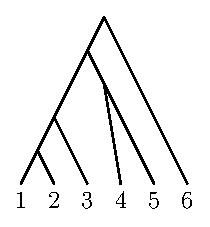
\includegraphics[width=0.25\textwidth]{ranked_tree}
\vspace{12pt}
\caption{A ranked tree with $6$ taxa.}
\label{fig:ranked_tree}
\end{figure}

In line with the research programme proposed in \autocite{Gavryushkin2018-ol}, we investigate the geometry and algorithmic complexity of the $\rnni$ space.
Specifically, in this paper we establish the exact radius and diameter of the space (Section~\ref{section:diameter}).
We also show that the subset of caterpillar trees is convex in $\rnni$ (Section~\ref{section:caterpillar_convex}), thus settling one of the open problems proposed in \autocite{Gavryushkin2018-ol}.
For establishing these geometric properties we are using algorithms that will be introduced in Section~\ref{section:algorithms}.
We will in particular provide an approximate algorithm that computes exact distances for small trees.
The question of whether there exists a polynomial algorithm for computing the $\rnni$ distance remains an open problem.

In the rest of this chapter we formally introduce the terminology used in this paper.

A \emph{ranked phylogenetic tree} is a pair consisting of a rooted binary phylogenetic tree $T$ on the set $X = \{1, \ldots, n\}$ of \emph{taxa} for $n \in \mathbb N$, and a (total) rank function that maps all leaves of $T$ to $0$, all internal nodes of $T$ onto elements of the set $\{1, \ldots, n-1\}$, and respects the partial order on the nodes given by the tree.
The latter means that if $u$ and $v$ are two internal nodes of $T$ such that there exists a path from a taxon $x \in X$ to the root which first passes through $u$ and then through $v$ then $\rank(u) < \rank(v)$.
Ranked trees $(T_1, \rank_1)$ and $(T_2, \rank_2)$ are different if trees $T_1$ and $T_2$ are different or $T_1 = T_2$ and $\rank_1 \neq \rank_2$.
Since all trees in this paper are ranked trees, we will abuse the notation and drop the rank function from the notation.
We will also simply say trees to mean ranked phylogenetic trees.
For a tree $T$, we will use $\rank_T$ to refer to its ranking.
A ranked tree $T$ without its leaf labels will be called \emph{tree topology}.

Our definition of a ranked tree implies a natural notion of edge length -- we call $|\rank_T(v) - \rank_T(u)|$ the length of an edge $(u, v)$.

Now we are ready to define the tree space which is the subject of study in this paper, the $\rnni$ graph.

The vertex set of the $\rnni$ graph is the set of all ranked trees on $n$ taxa.
We introduce two types of operation ($\rnni$ \emph{moves}) on trees (see Figure~\ref{fig:RNNI}) and say that two trees are adjacent in the $\rnni$ graph if they are connected by an operation of either type.
The first type of operation is called a \emph{rank move} and defined by swapping the ranks of two internal nodes that are not adjacent in the tree.
Formally, if $u$ and $v$ are nodes of a tree $T$ such that $|\rank_T(u) - \rank_T(v)| = 1$ and $(u, v)$ is not an edge in $T$ then the tree $R$ obtained from $T$ by only changing $\rank_R(u) = \rank_T(v)$ and $\rank_R(v) = \rank_T(u)$ is said to be obtained by a rank move.
The second type of operation is called an $\nni$ \emph{move} and defined in the usual way, that is, two trees $T$ and $R$ are said to be connected by an $\nni$ move if there exist internal edges $e$ in $T$ and $f$ in $R$ both of length one such that the trees obtained by shrinking $e$ and $f$ to internal nodes coincide.

We use the notation $d(T, R)$ throughout the paper to denote the graph distance between trees in $\rnni$, that is, $d(T, R)$ is the length of a shortest $\rnni$ path between tree $T$ and $R$.

\begin{figure}[H]
\centering
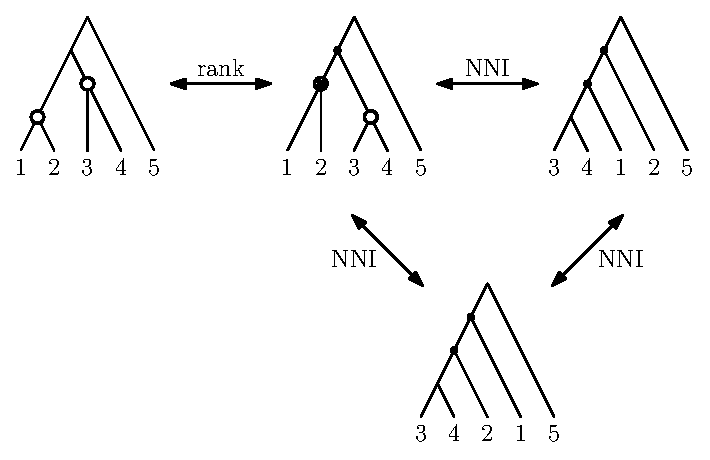
\includegraphics[width=0.8\textwidth]{RNNI}
\vspace{12pt}
\caption{Two types of operation that define edges of the $\rnni$ graph.
The rank move swaps the ranks of the two nodes in the tree on the left such that $\nni$ moves are possible on the edge between the two nodes marked by black dots.}
\label{fig:RNNI}
\end{figure}


\section{Algorithms}
\label{section:algorithms}

We start this section with a discussion of the algorithm proposed in \autocite{Gavryushkin2018-ol} to compute the exact $\rnni$ distance between trees by pre-computing the $\rnni$ graph.
Then we introduce two algorithms, $\findpath$ (Section~\ref{section:alg_findpath}) and $\csort$ (Section~\ref{section:alg_csort}), for computing paths between two given trees in $\rnni$.
These algorithms will become an important ingredient to establish several geometric properties of the $\rnni$ graph in Section~\ref{section:geometry}.
Finally we will present the algorithm $\mdtree$, which produces a tree that is far away from the given input tree (see Section~\ref{section:alg_mdtree} for details).
While this algorithm is interesting on its own (e.g.\ for simulation studies), we will again apply the algorithm to study the geometry of the $\rnni$ space.

For comparing approximate distances computed by $\findpath$ (Section~\ref{section:alg_findpath}) with exact distances and for supporting Conjecture~\ref{conjecture:cluster_theorem}, we aim to compute exact distances in $\rnni$ for small trees.
Therefore we will use the algorithm for computing the $\rnni$ graph that is given in \textcite[Section 3.3]{Gavryushkin2018-ol}.
\todo{Do we make use of tanglegrams? - LC: No}
\todo{GitHub link?}
Once the graph is computed one can use common algorithms for computing shortest paths~\autocite{Floyd1962-ew,Dijkstra1959-ph}.
However, the large number of vertices in $\rnni$ is an obstacle when it comes to computing distances.
Since there are $\frac{n!(n-1)!}{2^{n-1}}$ vertices in the $\rnni$ graph \autocite{Gavryushkin2018-ol}, we are just able to use the $\rnni$ graph on up to six taxa for our analyses.
We will get into further details when we discuss particular problems in Section~\ref{section:alg_findpath} and~\ref{section:cluster_theorem}.


\subsection{$\findpath$}
\label{section:alg_findpath}

Within this section we are presenting $\findpath$, an efficient algorithm for computing paths, and therefore approximating distances, between any given pair of trees in $\rnni$.
As we will see in Section~\ref{section:geometry}, it is useful for gaining insights into geometric properties of the $\rnni$ graph.

Before introducing the algorithm we need the following definitions.
Each node $v$ of a tree defines a \emph{cluster} $C$, which is the set of taxa descending from $v$.
We then say that $v$ \emph{induces} $C$.
\emph{Trivial clusters} are clusters induced by leaves (contain just one element each) and the root of the tree (contains all taxa).
As all trees on $n$ taxa share all trivial clusters, we will use the notion cluster to mean non-trivial clusters.
Note that the list of all non-trivial clusters of a tree, sorted according to the rank of the corresponding node, defines the tree unambiguously.
We will refer to this list of $n-2$ clusters for a given tree on $n$ taxa as a \emph{cluster representation} of the tree.

We are now ready to explain how $\findpath$ (Algorithm~\ref{alg:find_path}) computes a path between two input trees $T$ and $R$.
Let $[C_1, \ldots, C_{n-2}]$ be the cluster representation of $R$ (the ``destination'' tree).
Then $C_i$ is induced by the node of rank $i$ for $i = 1, \ldots, n-2$.
$\findpath$ computes a path which initially consists of $T_0 = T$ only and is extended stepwise as described in the following.

Step $0$.
$p = [T_0]$.
Consider the node in $T_0$ that induces the smallest cluster containing all elements of $C_1$.
This node is denoted by $\mrca_{T_0}(C_1)$ (short for \emph{most recent common ancestor}).
By performing an $\rnni$ move that decreases the rank of $\mrca_{T_0}(C_1)$, we receive a tree $T_1$ that is then appended to $p$.
Now we repeatedly perform $\rnni$ moves that move the most recent common ancestor of $C_1$ down in order to extend $p$ to $p = [T_0, \ldots, T_l]$ for some $l$ such that $C_1$ is induced by the internal node of rank one in $T_l$.

Step $k$.
$p = [T_0, \ldots, T_l]$ where $l$ is the total number of trees that have been added to $p$ in the previous $k-1$ steps.
Therefore the internal nodes in $T_l$ with ranks $1, \ldots, k-1$ induce clusters $C_1, \ldots, C_{k-1}$, respectively.
Now the cluster of interest is $C_k$.
As in the first step $p$ is extended by performing a series of $\rnni$ moves that decrease the rank of $\mrca_{T_l}(C_k)$ stepwise.
Afterwards it is $p = [T_0, \ldots, T_{l'}]$ where the $k$ lowest internal nodes of $T_{l'}$ induce clusters $C_1, \ldots, C_{k}$.

By following this procedure, the end tree of $p$ after step $n-2$ will be $R$, as it contains all clusters of $R$.
It is important but easy to see that the output path of $\findpath$ is unique for a given pair of trees, which means that it is a deterministic algorithm.
This is due to the fact that there exists exactly one $\rnni$ move that decreases the rank of the most recent common ancestor of a subset $C_k$ of the taxon set of a tree as long as $C_k$ is not induced by an internal node of that tree.

\todo{$p = p+T'$: Do we really want to be updating this in every while loop? - LC: Yes, I guess so}
\begin{algorithm}[H]
\caption{$\findpath$($T,R$)}
\label{alg:find_path}
\begin{algorithmic}[1]
\STATE $T' := T$
\STATE $p := [T']$
\FOR {$k = 1, \dots, n-2$}
\STATE Let $C_k$ be the cluster induced by the node with rank $k$ in $R$ \label{alg:find_path:line:cluster}
\WHILE {$\rank_{T'}(\mrca_{T'}(C_k))>k$}
\STATE Update $T'$: Decrease $\rank_{T'}(\mrca_{T'}(C_k))$ by an $\rnni$ move \label{alg:findpath:line:move_set_down}
\STATE $p = p+T'$
\ENDWHILE
\ENDFOR
\RETURN $p$
\end{algorithmic}
\end{algorithm}

The following lemma shows that $\findpath$ gives a path between the two input trees, indeed, by proving that there is always an $\rnni$ move possible as described in Line~\ref{alg:findpath:line:move_set_down} of Algorithm~\ref{alg:find_path}.

\begin{lemma}
Let $T = [C_1, \ldots, C_{k-1}, B_{k}, \ldots, B_{n-2}]$ and $R = [C_1, \ldots, C_{k-1}, C_k, \ldots, C_{n-2}]$ be two trees where $C_k \neq B_k, \ldots, B_{n-2}$.
Then there exists exactly one $\rnni$ move on $T$ that results in a tree $T'$ such that $\mrca_{T'}(C_k) < \mrca_{T}(C_k)$.
\label{lemma:mrca_move}
\end{lemma}

\begin{proof}
Let $T$ and $R$ be trees as defined in the lemma.
Notice that the only $\rnni$ move on $T$ that could decrease the rank of $\mrca_T(C_k)$ are $\nni$ moves on the edge between $\mrca_T(C_k)$ and its child (if this edge has length one), or a rank move between $\mrca_T(C_k)$ and the node with rank one less.
Therefore, we will now distinguish these two cases:
Either there is an edge $(v,w)$ between nodes $v = \mrca_T(C_k)$ and $w$ with rank $rank_T(w) = rank_T(v) - 1$, or there is no such edge.

In the latter case the only $\rnni$ move that could decrease the rank of $v$ is a rank move swapping the ranks of $v$ and $w$.

Let us now assume that there is an edge $(v,w)$ in $T$.
Let $T_v$ be the subtree that is rooted in the child of $v$ that is not $w$ and let $T_{w_1}$ and $T_{w_2}$ be the subtrees rooted in the children of $w$.
We are now going to explain why only one of these two $\nni$ moves changes the rank of $\mrca_T(C_k)$.
It is important to notice that $C_k$ either is the disjoint union of two of the clusters $C_1, \ldots, C_{k-1}$ or the union of one of those clusters with a single taxon that is not included in any of those clusters.
In general we can say that $C_k = S_1 \dot\cup S_2$ is the union of two subsets of taxon set of $T$ such each of these subsets is contained in one of the subtrees $T_v, T_{w_1}$, or $T_{w_2}$.
In fact, $S_1$ and $S_2$ are contained in two different of these subtrees.
Now it is easy to see that just one of the $\nni$ moves on $(v,w)$ (illustrated in Figure~\ref{fig:mrca_move}) decreases the rank of $\mrca_T(C_k)$.

% It is important to notice that $C_k$ either is the disjoint union $C_k = C_i \dot\cup C_j$ for $i,j < k$ or $C_k = C_i \dot\cup \{x\}$ for a taxon $x \in X \setminus (C_1 \cup \ldots \cup C_{k-1})$.
%
% Let us at first assume that $C_k = C_i \dot\cup C_j$ for some $i,j < k$.
% The tree $T$ looks like the tree depicted in the left of Figure~\ref{fig:mrca_move} where $T_w^1$ and $T_w^2$ are the two subtrees rooted in the children of $w$ and $T_v$ is the subtree whose root is child of $v$ and does not include $w$.
% Since we know that all clusters $C_1,\ ldots, C_{k-1}$ are induced by some nodes in $T$, each of these clusters must be a subset of the taxon set of one of the three subtrees $T_w^1,T_w^2$, or $T_v$.
% In particular, there can't be elements of the same cluster $C_m$ in more than one of these subtrees.
% This and the fact that $v = \mrca_{T}(C_i \dot\cup C_j)$ yields that either $C_i$ or $C_j$ is subset of the taxon set of $T_v$ and the other cluster is subset of the taxon set of either $T_w^1$ or $T_w^2$.
%
% Without loss of generality we assume that $C_i$ is included in $T_v$.
% Otherwise, change the indices $i$ and $j$.
% Then $C_i$ is a subset of the taxon set of either $T_w^1$ or $T_w^2$.
% Therefore, just one of the two $\nni$ moves on $(v,w)$, as depicted in Figure~\ref{fig:mrca_move}, moves the most recent common ancestor of $C_k = C_i \dot \cup C_j$ down.
%
% Now we consider the case that $C_k = C_i \dot\cup \{x\}$ for a taxon $x \in X \setminus (C_1 \cup \ldots \cup C_{k-1})$.
% For the same reason as above, $C_i$ is in subset of the taxon set of one of the subtrees $T_w^1, T_w^2$ or $T_v$ of $\hat T$ as depicted in Figure~\ref{fig:mrca_move}.
% Similarly $x$ is taxon of one of these three subtrees in a way that either $C_i$ or $x$ is included in $T_v$, because $v = \mrca_{T'}(C_i \dot \cup \{x\})$.
% So there is just one of the two subtrees $T_w^1$ and $T_w^2$ that neither includes $C_j$ nor $x$.
% As in the previous case, just one of the two $\nni$ moves on $(v,w)$ as illustrated in Figure~\ref{fig:mrca_move} decreases the rank of $\mrca_{T}(C_i \dot \cup \{x\})$.
%
% We can conclude that in any case there is exactly one $\rnni$ move possible on $T$ that decreases the rank of $\mrca_{T}(C_k)$ in Line~\ref{alg:findpath:line:move_set_down} of Algorithm~\ref{alg:find_path}.

\begin{figure}[H]
\centering
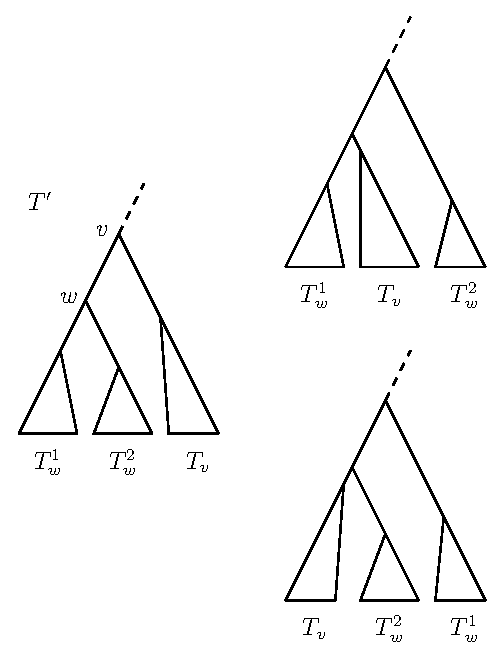
\includegraphics[width=0.5\textwidth]{mrca_move}
\vspace{12pt}
\caption{Two $\nni$ moves that are possible on the edge $(v,w)$ of the tree $T'$ with subtrees $T_v, T_{w_1}, T_{w_2}$ as described in the proof of Lemma~\ref{lemma:mrca_move}.}
\label{fig:mrca_move}
\end{figure}

\end{proof}

Note that the uniqueness of the $\rnni$ move in Line~\ref{alg:findpath:line:move_set_down} of Algorithm~\ref{alg:find_path} implies that the algorithm is deterministic.
The running time of the algorithm is quadratic in the number of taxa.

Because the algorithm returns a path between pairs of trees in $\rnni$, the length of the path approximates the $\rnni$ distance from above.
A natural question then is how accurate this approximation is.
To answer this question for small trees, we have implemented the algorithm $\findpath$
\todo{LC: github - link}
\autocite{}
and compared the results with the true distance found using the algorithm from Section~\ref{section:algorithms}.
By doing this we could show that $\findpath$ computes correct distances for all trees on up to six taxa.

\subsection{$\csort$}
\label{section:alg_csort}

In this section we introduce an algorithm to compute paths between \emph{caterpillar trees}, which are trees where each internal node is adjacent to at least one leaf.
As a result caterpillar trees have only one \emph{cherry}, which is a pair of taxa that share their parent.
For introducing this algorithm we need the following definitions.
A path $p$ between two caterpillar trees $T$ and $R$ that only consists of caterpillar trees is called a \emph{caterpillar path}.
If $p$ is the shortest path among all caterpillar paths between $T$ and $R$ we call it a \emph{shortest caterpillar path}, and denote the length of $p$ by $d_c(T,R)$, which we call the \emph{caterpillar distance}.

The special topology of caterpillar trees gives a natural preorder of taxa that uniquely represents a caterpillar tree.
That is, for a caterpillar tree $T = [\{x_1, x_2\}, \{x_1, x_2, x_3\}, \ldots, \{x_1, \ldots, x_n\}]$ the taxa are preordered according to the ranks of their parents such that $x_1 = x_2 \leq x_3 \leq \ldots \leq x_n$.
From now on when we say that a taxon is below another one we refer to this preorder.
Furthermore, we can use this preorder to create a list representation of caterpillar trees.
For the tree $T$ above this list is $[x_1, x_2, \ldots, x_n]$.
As we consider the taxon set $X = \{1, \ldots, n\}$, we assume that they are ordered in the list such that $x_1 < x_2$, according to their ordering as natural numbers.
This ensures that the list representation of caterpillar trees is unique.

%We are now going to explain what kind of $\rnni$ moves are possible between caterpillar trees and see how such a move changes the list representation of a tree.
%At first it is important to realise that the only possible $\rnni$ moves between caterpillar trees are $\nni$ moves, since there is no pair of internal nodes with rank difference one that is not connected by an edge.
%$\nni$ moves between caterpillar trees correspond to swaps of two neighboured elements in the list representation.
%The only exception of this are $\nni$ moves on the lowest internal edge, that is the edge connecting the internal nodes of rank one and two.
%There are two $\nni$ moves possible on this edge that result in caterpillar trees, while there is for every other edge only one $\nni$ move that results in a caterpillar tree.
%Corresponding to the $\nni$ moves on the lowest internal edge are exchanges of either the first or the second element with the third element in the list representation.

The algorithm $\csort$ (Algorithm~\ref{alg:csort}) is a natural modification of the classical \emph{Bubble Sort} algorithm \autocite{Knuth1997-pi}.
A path $p$ between two given trees $T$ and $R$ is computed by sorting the list representations of $T$ and $R$ as it is done in Bubble Sort.
The general idea is to update the list representing $T$ by considering it from beginning to end and swap two neighboured taxa if they appear in a different order in $R$ than in the current list.
Note that each swap of taxa results in a new tree that is added to the path $p$.
After passing the whole list the last element, which is the uppermost taxon, is at the same position as in $R$.
By repeating this at most $n-1$ times all elements the resulting list represents $R$.

We use this main principle of Bubble Sort for computing shortest caterpillar paths with $\csort$, but there are special consideration needed for the first three taxa.
The reason for this is that both $\nni$ moves on the lowest internal edge of a caterpillar tree result in caterpillar trees.
For computing a shortest caterpillar path the moves on the first three taxa $x_1, x_2, x_3$ need to be done as described in the following.
If $x_1$ ($x_2$) is the uppermost taxon of those three in $R$, we update the current tree by swapping $x_1$ ($x_2$) and $x_3$.
By doing this we make sure that there will be no point on $p$ where $x_1$ and $x_2$ swap positions, as this is an additional $\nni$ move that can be avoided.

Because all moves between caterpillar trees are $\nni$ moves, all pairs of taxa that are not in the same order in $T$ and $R$ need to swap at some point on any path between these trees.
And since only elements that are direct neighbours in a sequence are allowed to swap, with the only exception being the first three elements, the path computed by $\csort$ is a shortest caterpillar path indeed.

\begin{algorithm}[H]
\caption{$\csort$($T,R$)}
\label{alg:csort}
\begin{algorithmic}[1]
\STATE $T':= T$, $p := [T']$
\STATE $L_{T'}:=$ list representation of $T'$, $L_R:=$ list representation of $R$
% \STATE $L_{\hat T} :=$ list representation of $\hat T$, $L_R :=$ list representation of $R$
\FOR {$i=1,\ldots,n-2$} \label{alg:csort:line:loop}
\STATE $j = 0$ \COMMENT{Special case: cherry}
\IF {$L_{T'}[0]$ is last element of $L_{T'}[0],L_{T'}[1],L_{T'}[2]$ in $L_R$}
\STATE Update $T'$: swap $L_{T'}[0]$ and $L_{T'}[2]$
\ELSIF {$L_{T'}[1]$ is last element of $L_{T'}[0],L_{T'}[1],L_{T'}[2]$ in $L_R$}
\STATE Update $\hat T$: swap $L_{T'}[1]$ and $L_{T'}[2]$
\ENDIF
\STATE $j = 2$
% \IF {$L_R^{-1}[L_{\hat T}[j]] > L_R^{-1}[L_{\hat T}[j+1]]$}
\WHILE {order of $L_{T'}[j]$ and $L_{T'}[j+1]$ different in $R$}
\STATE Update $T'$: Swap $L_{T'}[j]$ and $L_{T'}[j+1]$
\STATE $p = p+T', j = j + 1$
\ENDWHILE
\ENDFOR
\RETURN $p$
\end{algorithmic}
\end{algorithm}

The running time of $\csort$ is the same as for Bubble Sort, that is quadratic in $n$.
Though simple, this algorithm will be crucial for some proofs in Section~\ref{section:caterpillar_convex}.


\subsection{$\mdtree$}
\label{section:alg_mdtree}

The algorithm we are going to introduce here will be important for finding the radius of the $\rnni$ graph.
It is called $\mdtree$, which stands for Maximum Distance Tree, as it computes a tree with maximum distance if the input tree is a caterpillar tree.
This will be discussed in Section~\ref{section:diameter}.

$\mdtree$ (Algorithm~\ref{alg:max_dist_tree}) works as follows:
At first, all taxa of the input tree $T$ are sorted in a list $L = [l_1, \ldots, l_n]$ such that the ranks of their parents are non-decreasing.
Though this representation appears similar to the list representation of caterpillar trees, it is ambiguous since we do not specify how to order cherry taxa.
$\mdtree$ constructs an output tree $R$ as follows:
Initially, $R$ only consists of a cherry with taxa $l_1$ and $l_2$ such that the parent of these taxa has rank $n-1$.
The remaining taxa are added to $R$ sequentially, according to their order in $L$, by creating a new internal node at one of the existing branches in $R$ such that this new node has rank one less than the previously lowest internal node in $R$.

\begin{algorithm}[H]
\caption{$\mdtree(T)$}
\label{alg:max_dist_tree}
\begin{algorithmic}[1]
\STATE Construct list $L=[l_1, \ldots, l_n]$ of all taxa, ordered such that the ranks of their parents in $T$ do not decrease \label{alg:mdtree_lineL}
\STATE Build tree $R$ with only two taxa $l_1, l_2$ that are children of the root, an internal node with rank $n-1$
\FOR {$i = 1, \ldots, n$}
\STATE Add an internal node as parent of $l_i$ on an edge in $R$ such that the new internal node has rank one less than the previously lowest internal node \label{alg:mdtree_lineAddTaxon}
\ENDFOR
\RETURN $R$
\end{algorithmic}
\end{algorithm}

Both the list computed in Line~\ref{alg:mdtree_lineL} the and the attachment edge of the new taxon in the tree in Line~\ref{alg:mdtree_lineAddTaxon} are not uniquely determined within $\mdtree$.
Therefore, this algorithm is non-deterministic which is an important observation needed in Section~\ref{section:diameter} where this algorithm is used for finding the radius of $\rnni$.

\section{Geometry of $\rnni$}
\label{section:geometry}

In this section we analyse shortest paths in $\rnni$.
Therefore, we will use the algorithms introduced in the previous section.
They enable us to prove that there is always a shortest path between two caterpillar trees that only consists of caterpillar trees (Theorem~\ref{thm:caterpillar_convex}) in Section~\ref{section:caterpillar_convex}.
In other words, the set of caterpillar trees is \emph{convex} in $\rnni$.
In Section~\ref{section:diameter} we will investigate diameter and radius of the $\rnni$ graph.
Interestingly, the \emph{diameter} of $\rnni$, that is the maximum distance $\Delta(\rnni) = \max \{d(T, R) \mid T, R \in \rnni\}$ between any two trees in the graph, equals its \emph{radius} $rad(\rnni) = \min\limits_T \max\limits_R d(T,R)$.
After proving this, we are going to consider the so-called Split Theorem, which was raised in \autocite{Gavryushkin2018-ol}.
We will give a counterexample to disprove their version of the Split Theorem and claim an alternative version, the Cluster Theorem (Conjecture~\ref{conjecture:cluster_theorem}).

Before we get into the details of these geometric properties of $\rnni$, we need to prove some statements that will be used a few times within this geometry section.

\begin{lemma}
It is $\Delta(\rnni) \leq \frac{(n-1)(n-2)}{2}$ for $n \geq 3$.
\label{lemma:diameter_bound}
\end{lemma}

\begin{proof}
Since the diameter is bounded from above by the maximum length of a path computed by $\findpath$, it is enough to find this maximum.
Let us assume that $T$ and $R = [C_1, \ldots, C_{n-2}]$ are trees for which $\findpath$ computes a path of maximum length.
That means that if $T'$ is the last tree of $p$ at the beginning of loop number $i$ in the execution of $\findpath(T,R)$, $\mrca_{T'}(C_i)$ is the root.
Thus, there are $n-1-i$ $\rnni$ operations needed to move $C_i$ to its correct position.
Hence, the maximum length of a path computed by $\findpath$ is bounded by $\sum\limits_{i = 1}^{n-2} n-1-i = \frac{(n-2)(n-1)}{2}$.
\end{proof}

The following lemma relates distances between trees on $n$ and $n+1$ taxa and is an important tool for inductive arguments.
We use the notion $\parent_T(x)$ to refer to the node adjacent to taxon $x$ in tree $T$.
$T{\big|}_n$ denotes the restriction of tree $T$ to the set of taxa $\{1, \ldots, n\}$.
In particular if $T$ is a tree on taxa $\{1, \ldots, n+1\}$ the tree $T{\big|}_n$ is obtained by deleting taxon $n+1$ and suppressing the thereby created node of degree two.

\begin{lemma}
Let $T$ and $R$ be two trees on taxa $\{1, \ldots, n+1\}$.
Then $d(T{\big|}_n, R{\big|}_n) \leq d(T,R) - \delta$, where $\delta = |\rank_T(\parent_T(n+1)) - \rank_R(\parent_R(n+1))|$.
\label{lemma:distance_delete_taxon}
\end{lemma}

\begin{proof}
Let $T$ and $R$ be trees as described in the lemma.
First observe that the rank of the internal node $\parent_T(n+1)$ can only be changed by performing a rank move that involves $\parent_T(n+1)$ or an $\nni$ move on an edge adjacent to $\parent_T(n+1)$.
Second observe that any $\rnni$ move can change the rank of $\parent_T(n+1)$ by at most one.
So we can follow that an $\rnni$ move on $T$ can decrease the rank of $\parent_T(n+1)$ by at most one.

Let $p$ be a shortest path from $T$ to $R$ and $p{\big|}_n$ the path resulting from deleting taxon $n+1$ from all trees on $p$.
Then $p{\big|}_n$ is a path from $T{\big|}_n$ to $R{\big|}_n$.
The reason for this is that the only moves that are deleted from $p$ to receive $p{\big|}_n$ are those involving the parent of taxon $n+1$.
All other moves stay the same and can be performed equally on a path from $T{\big|}_n$ to $R{\big|}_n$ as on a path from $T$ to $R$, because the relations of all other internal nodes are the same between both pairs of trees.
Recall that $\delta$ is the difference in ranks between the parents of taxon $n+1$ in $T$ and $R$.
With the knowledge that an $\rnni$ move on $T$ can change the rank of $\parent_T(n+1)$ by at most one, we can conclude that $|p{\big|}_n| \leq |p| - \delta$.
Since $d(T{\big|}_n,R{\big|}_n) \leq |p{\big|}_n|$ and $|p| = d(T,R)$, the desired inequality follows.
\end{proof}


\subsection{The set of caterpillar trees}
\label{section:caterpillar_convex}

In this section we restrict our attention to the set of caterpillar trees.
Throughout this section the simplified list representation for these trees as introduced in Section~\ref{section:alg_csort} will be used.
This type of tree is of particular interest in $\rnni$ because shortest paths between such trees in $\rnni$ differ from those in classical $\nni$ space.
Following this observation and the importance of caterpillar trees in the proof of $\np$-hardness of $\nni$ distances in \autocite{Dasgupta2000-xa}, understanding the geometry of paths between caterpillar trees seems essential for investigating the complexity of computing $\rnni$ distances.
In the following we demonstrate why finding shortest paths between caterpillar trees builds the basis for understanding the difference between $\nni$ and $\rnni$.

Let us compare shortest paths between caterpillar trees in $\nni$ with those in $\rnni$.
It can happen in $\nni$ that building a cherry and moving it may give a path that is shorter than a path where the taxa move separately in as it is illustrated out in Figure~\ref{fig:NNI_vs_RNNI}.
There is only one move needed to build and resolve a cherry, respectively, while the number of moves for moving the cherry is the same as for moving a single taxon in $\nni$.
In $\rnni$ space however, there are additional rank moves needed to change the rank of the internal node of the cherry before an $\nni$ move can resolve it.
This is due to the fact that $\nni$ moves are only allowed on edges of length one in $\rnni$.
As a consequence a path where taxa move separately and no new cherry is built is shortest in $\rnni$.

\begin{figure}[H]
\centering
\includegraphics[width=\textwidth]{NNI_vs_RNNI}
\vspace{12pt}
\caption{Paths between caterpillar trees $T$ and $R$: The solid paths are paths in $\rnni$, the dashed one is a path that is only possible in the plain $\nni$ graph.
The upper path is a natural extension of the shortest $\nni$ path in $\rnni$.
It is longer than a shortest $\rnni$ path as the one at the bottom which consists of caterpillar trees only.}
\label{fig:NNI_vs_RNNI}
\end{figure}

The above observation suggests that there is a caterpillar path that is a shortest path between any two caterpillar trees in $\rnni$.
Indeed, we are going to prove within this section that the set of caterpillar trees is convex in $\rnni$ (Theorem~\ref{thm:caterpillar_convex}).
Note that this is not true for the $\nni$ space, which is clear from the example in Figure~\ref{fig:NNI_vs_RNNI}.

The following lemma regards caterpillar trees with distance $\frac{(n-1)(n-2)}{2}$ and will be needed for proving the convexity of the set of caterpillar trees in $\rnni$.
Notice that $\frac{(n-1)(n-2)}{2}$ is the upper bound for the diameter of $\rnni$ by Lemma~\ref{lemma:diameter_bound}.

\begin{lemma}
Let $T$ and $R$ be two caterpillar trees.
$T$ and $R$ have distance $d(T,R) = \frac{(n-1)(n-2)}{2}$ if, and only if, they have caterpillar distance $d_c(T,R) = \frac{(n-1)(n-2)}{2}$.
\label{lemma:caterpillar_dist=diameter}
\end{lemma}

\begin{proof}
Let $T$ and $R$ be caterpillar trees.
Let us first prove that if $d(T,R) = \frac{(n-1)(n-2)}{2}$, it follows $d_c(T,R) = \frac{(n-1)(n-2)}{2}$.
This easily follows from algorithm $\csort$:
In each loop $i=1, \ldots, n-2$ of $\csort$ (Algorithm~\ref{alg:csort}) there are at most $n-1-i$ pairs of taxa that swap positions.
This is due to the fact that after loop number $i$ the last $i$ elements in the list representation of the current tree on $p$ are in the same place as in the destination tree.
As a result there are no further exchanges of pairs of taxa within the last $i-1$ taxa of the tree in loop $i$, which means that at most $n-1-i$ pairs of taxa exchange then.
It follows that the maximum length of a path computed by $\csort$ is $\sum\limits_{i=1}^{n-2} n-1-i = \frac{(n-1)(n-2)}{2}$.
Since there cannot be a caterpillar path shorter than $d(T,R) = \frac{(n-1)(n-2)}{2}$, it follows $d_c(T,R) = \frac{(n-1)(n-2)}{2}$.

For proving the other direction of the statement, let now $T$ and $R$ have caterpillar distance $d_c(T,R) = \frac{(n-1)(n-2)}{2}$.
We prove $d(T,R) = \frac{(n-1)(n-2)}{2}$ by induction on the number of taxa $n$ of $T$ and $R$:

Induction basis: $n=3$\\
There are three trees on three taxa.
They all have distance one from another and are caterpillar trees.
So it is $d(T,R) = d_c(T,R) = 1$ for all pairs of trees $T,R$ on $n=3$ taxa.

Induction step: $n \to n+1$\\
Induction hypothesis: For caterpillar trees $T, R$ on $n$ taxa with caterpillar distance $d_c(T,R) = \frac{(n-1)(n-2)}{2}$ it is $d(T,R) = \frac{(n-1)(n-2)}{2}$.\\
Without loss of generality we can assume that $T$ is the caterpillar tree $[1,2,3,\ldots,n+1]$.
Let $R$ be a caterpillar tree with distance $\frac{n(n-1)}{2}$ to $T$.
It follows that in each loop of $\csort$ the maximum number of taxon swaps is reached which implies that every taxon will swap with taxon $n+1$ at some point.
We can conclude that this taxon $n+1$ is part of the cherry of $R$.
Let us now consider the trees $T{\big|}_n$ to $R{\big|}_n$ that result from $T$ and $R$ by deleting taxon $n+1$.
$\csort$ computes a path from $T{\big|}_n$ to $R{\big|}_n$ that contains the same exchanges of taxa as $p$, except for the $n-1$ ones on $p$ that involve taxon $n+1$.
Hence, the caterpillar distance is $d_c(T{\big|}_n, R{\big|}_n) = \frac{n(n-1)}{2} - (n-1)$ = $\frac{(n-1)(n-2)}{2}$.
So we can apply the induction hypothesis on $T{\big|}_n$ and $R{\big|}_n$ and know that $d(T{\big|}_n,R{\big|}_n) = \frac{(n-1)(n-2)}{2}$.

We are now using this observation to prove that the distance between $T$ and $R$ equals $\frac{n(n-1)}{2}$.
This obviously gives an upper bound for the distance as it is $\Delta(\rnni_{n+1}) \leq \frac{n(n-1)}{2}$ for the $\rnni$ graph on $n+1$ taxa by Lemma~\ref{lemma:diameter_bound}.
It is left to prove that $\frac{n(n-1)}{2}$ is a lower bound for the distance between $T$ and $R$ as well.
According to Lemma~\ref{lemma:distance_delete_taxon}, the distance between $T{\big|}_n$ and $R{\big|}_n$ is at least $d(T{\big|}_n, R{\big|}_n) \leq d(T,R) - |\rank_T(\parent_T(n+1)) - \rank_R(\parent_R(n+1))|$.
We also know $|\rank_T(\parent_T(n+1)) - \rank_R(\parent_R(n+1))| = n-1$.
Suppose, contrary to our claim, that there is a path from $T$ to $R$ of length less than $\frac{n(n-1)}{2}$.
By the above, it follows that $d(T{\big|}_n, R{\big|}_n) \leq d(T,R) - |\rank_T(\parent_T(n+1)) - \rank_R(\parent_R(n+1))| < \frac{n(n-1)}{2} - (n-1) < \frac{(n-1)(n-2)}{2}$.
Since this is a contradiction to $d(T{\big|}_n, R{\big|}_n) = \frac{(n-1)(n-2)}{2}$, it is proven that $d(T,R) = \frac{n(n-1)}{2} $.
\end{proof}

\begin{theorem}
The set of caterpillar trees is convex.
\label{thm:caterpillar_convex}
\end{theorem}

\begin{proof}
We prove this Theorem by backwards induction on the caterpillar distance $l = d_c(T,R)$ between caterpillar trees $T$ and $R$.
For this backwards induction the maximum caterpillar distance $\frac{(n-1)(n-2)}{2}$ (Lemma~\ref{lemma:caterpillar_dist=diameter}) is the base case.

Induction basis: $l = \frac{(n-1)(n-2)}{2}$\\
With Lemma~\ref{lemma:caterpillar_dist=diameter} one can see that for each pair of caterpillar trees $T$, $R$ with caterpillar distance $d_c(T,R) = \frac{(n-1)(n-2)}{2}$, it is $d(T,R) = d_c(T,R)$.
Thus there is a shortest path between $T$ and $R$ that is a caterpillar path.

Induction step: $l+1 \to l$\\
Induction hypothesis: For each pair of caterpillar trees with caterpillar distance $l+1$ there is a shortest path between these trees that consists of caterpillar trees only, so the distance between these trees is $l+1$.

Let $T$ and $R$ be caterpillar trees with caterpillar distance $l$.
We consider the shortest caterpillar path between these trees computed by $\csort$.
From now on we will consider the trees $T$ and $R$, as well as all other caterpillar trees within this proof, in their list representation $L_T$ and $L_R$ as introduced in Section~\ref{section:alg_csort}.

Since $l < \frac{(n-1)(n-2)}{2}$, there must be a loop in $\csort$ (Line~\ref{alg:csort:line:loop} of Algorithm~\ref{alg:csort}) where not every pair of taxa that is compared exchanges.
Let us consider the first pair of taxa $a,b$ that is compared but does not swap positions, where $a$ is below $b$.
Since the first time that this happens, $a$ is either one of the first two elements in the sequence, or it previously swapped with an element $c$ that has been between $a$ and $b$ before.

We start with considering the latter case.
The list representation of the tree at the point where $a$ and $b$ are compared but not swapped, looks as follows:
\[[\ldots, c, a, b, \ldots, x_k, \ldots, x_1]\]

Note that here we assume that the elements $x_1, \ldots, x_k$ are in the same place as they are in the destination tree $R$.
It could be that $k=1$, which means that there are no such elements.

Since $a$ and $c$ swap, but $a$ and $b$ do not, we can follow that $b$ and $c$ appear in $R$ in the same order as they do in the current tree.
Furthermore, $c$ and $b$ must have been neighbours in $T$, because we assume that the comparison of $a$ and $b$ is the first one where the compared elements are not swapped in the sequence.
Let now $\hat T$ be a tree that equals $T$ with the only exception that $b$ and $c$ are exchanged.
We can follow from our observations above that the distance between $T$ and $\hat T$ is $d(T, \hat T) = 1$ and that $\csort$ needs one move more for a path from $\hat T$ to $R$ than from $T$ to $R$.
This results in $d_c(\hat T, R) = d(T,R) + 1$.

So we can apply the induction hypothesis on $\hat T$ and $R$ and see that $d(\hat T,R) = l+1$.
If it now were $d(T,R) < l$, it would hold $d(\hat T,R) \leq d(T,R) + d(T,\hat T) < l + 1$ which contradicts the induction hypothesis.
We can conclude $d(T,R) = l$, which completes the proof for the case that $a$ is not one of the first two elements of $L_{T'}$.

Let us now consider the other case:
of the two taxa that are compared but do not swap positions, one is part of the cherry current tree.
Let $a$ and $b$ be the cherry taxa and $c$ their neighbour such that neither $a$ nor $b$ echanges with $c$.
Then the list looks like this:
\[[a, b, c, \ldots, x_k, \ldots, x_1]\]

If there is no swap of either $a$ or $b$ with $c$, we can construct a tree $\hat T$ with caterpillar distance $d_c(\hat T, R) = l+1$ and $d(T,\hat T) = 1$ in a similar way as in the previous case.
In the list representing the start tree $T$, either $a$ or $b$ must be neighbour of $c$.
This is due to the fact that we are currently considering the first comparison of elements where there is no swap.
We can assume without loss of generality that $a$ is neighbour of $c$ in $T$.
Then an exchange of $a$ and $c$ in $T$ yields a tree $\hat T$ with the desired properties.
As in the previous case we can then apply the induction hypothesis on $\hat T$ and conclude that there is a shortest path between $T$ and $R$ that only consists of caterpillar trees.
\end{proof}


\subsection{Diameter and radius}
\label{section:diameter}

With the results of Section~\ref{section:caterpillar_convex} we can easily get the exact diameter of the $\rnni$ graph and hence improve the bounds for the diameter given in Theorem 7 of \autocite{Gavryushkin2018-ol}.
In the following we show that the upper bound of the diameter provided by Lemma~\ref{lemma:diameter_bound} actually is the exact diameter of $\rnni$.

\begin{lemma}
There are two caterpillar trees in $\rnni$ with distance $\frac{(n-1)(n-2)}{2}$.
\label{lemma:caterpillar_diameter}
\end{lemma}

\begin{proof}
Let $T = [1,2,3,\ldots,n]$ and $R = [n-1,n,n-2,n-3, \ldots, 1]$ be two caterpillar trees.
According to Theorem~\ref{thm:caterpillar_convex}, there is a shortest path between $T$ and $R$ that is a caterpillar path.
We can compute a shortest caterpillar path by using $\csort$ as explained in Section~\ref{section:caterpillar_convex}.
When running this algorithm to compute a path from $T$ to $R$, each taxon $i$ ($i = 1, \ldots, n-1$) swaps $n-1-i$ times with its upper neighbour.
Therefore, the length of a shortest caterpillar path is $\sum\limits_{i=1}^{n-1}(n-1-i)  = \frac{(n-1)(n-2)}{2}$.
\end{proof}

\begin{corollary}
It is $\Delta(\rnniu) = \frac{(n-1)(n-2)}{2}$.
\label{corollary:diameter}
\end{corollary}

We now proceed to show that the radius of the $\rnni$ graph equals its diameter.
Therefore we use the algorithm $\mdtree$ that has been introduced in Section~\ref{section:alg_mdtree}.
Note that the results provided in this section are only true if the input tree of $\mdtree$ is a caterpillar tree.

\begin{lemma}
Let $T$ be a caterpillar tree.
Any tree $R = \mdtree(T)$ has distance $d(T,R) = \Delta(\rnni)$ to $T$.
\label{lemma:max_dist_caterpillar}
\end{lemma}

\begin{proof}
Recall that with Corollary~\ref{corollary:diameter} we know that $\Delta(\rnni) = \frac{(n-1)(n-2)}{2}$.
Within this proof we assume, without loss of generality, that it is $T = [1,2,3,\ldots,n]$.
We prove the lemma by induction on the number of taxa $n$.

Induction basis: $n = 3$\\
$\mdtree(T)$ results either in $R =[1,3,2]$ or $R'= [2,3,1]$ for $T = [1,2,3]$.
Since it is $d(T,R) = d(T,R') = 1 = \Delta(\rnni_3)$, the lemma is true for trees on $n=3$ taxa.

Induction step: $n \to n+1$\\
Induction hypothesis: For a caterpillar tree $T$ on $n$ taxa $\mdtree$ computes a tree $R$ with distance $d(T,R) = \frac{(n-1)(n-2)}{2}$.\\
Let us now assume that $T$ is a tree on $n+1$ taxa.
In the list $L$ computed in $\mdtree$ (Line~\ref{alg:mdtree_lineL} of Algorithm~\ref{alg:max_dist_tree}) taxon $n+1 $ is the last one as its parent, the root, has the highest rank in $T$.
This means that this taxon $n+1$ is the last one added to $R$ as in Line~\ref{alg:mdtree_lineAddTaxon} of this algorithm and therefore, it has parent with rank one in $R$.
Because the parent of $n+1$ has rank $n$ in $T$ and rank $1$ in $R$, we can conclude from Lemma~\ref{lemma:distance_delete_taxon} that for $T$ and $R$ restricted to taxa $1,\ldots,n$ it holds: $d(T|_n,R|_n) \leq d(T,R) - (n-1)$.
It is not hard to see that $R|_n$ can be received from $T|_n$ by applying $\mdtree$:
$R|_n$ can be constructed from input tree $T|_n$ in the same way as $R$ can be constructed from $T$, since the list $L$ computed in Line~\ref{alg:mdtree_lineL} of Algorithm~\ref{alg:max_dist_tree} for $T|_n$ is the same as the one for $T$, but without the last element.
So we can follow from the induction hypothesis and Lemma~\ref{lemma:distance_delete_taxon} that it is $d(T,R) \geq d(T|_n,R|_n) + (n-1) = \frac{(n-1)(n-2)}{2} = \frac{n(n-1)}{2}$, which concludes the proof of the lemma.
\end{proof}

In Section~\ref{alg:max_dist_tree} we already discussed that $\mdtree$ is a non-deterministic algorithm.
In fact, the output tree of $\mdtree$ can have any tree topology, since there is no restriction on where to add the new taxon in the already existing tree (Line~\ref{alg:mdtree_lineAddTaxon} of Algorithm~\ref{alg:max_dist_tree}).
This means that for each caterpillar input tree $\mdtree$ can compute a tree with any tree topology that has maximum distance from the input tree.
And as permuting labels of trees does not change the distance between them, there is for every tree $R$ on $n$ taxa a caterpillar tree $T$ with distance $d(T,R) = \Delta(\rnni) = \frac{(n-1)(n-2)}{2}$.
By this we obtain Corollary~\ref{corollary:radius}.

\begin{corollary}
The radius of the $\rnni$ graph is $rad(\rnni) = \Delta(\rnni) = \frac{(n-1)(n-2)}{2}$.
\label{corollary:radius}
\end{corollary}


\subsection{Cluster Theorem}
\label{section:cluster_theorem}

Within this section we will make a further step towards understanding the complexity of computing shortest paths in $\rnni$.
Since the problem of computing distances in the most common tree spaces as $\nni$ \autocite{Dasgupta2000-xa}, rooted $\spr$ \autocite{Bordewich2005-nx}, or $\tbr$ \autocite{Allen2001-ky} is known to be $\np$-hard, it is desirable to find a tree space that is less complex.
So far it is not known whether computing distances in $\rnni$ is $\np$-hard or not.
The natural approach to solve this question is to compare $\rnni$ and $\nni$ graph to see whether the proof of $\np$-hardness of $\nni$ applies to $\rnni$ as well.
Within this section we will explain why this is not the case.
Therefore we consider an example of shortest paths in $\nni$ that builds the key of the proof of its $\np$-hardness and explain why this example cannot be transferred to $\rnni$.
Following this, we will introduce the so-called Split Theorem (Conjecture~\ref{conjecture:split_theorem}), which has been conjectured in \autocite{Gavryushkin2018-ol}.
However, we present a counterexample disproving the Split Theorem in its original version and claiming the Cluster Theorem (Conjecture~\ref{conjecture:cluster_theorem}) as alternative version.

The proof of $\np$-completeness of $\nni$ in \autocite{Dasgupta2000-xa} is based on the fact that Theorem~\ref{thm:split_nni} holds for $\nni$.

\begin{theorem}
There are trees $T,R$ in $\nni$ sharing a cluster which is not shared by any intermediate tree on any shortest path from $T$ to $R$.
\label{thm:split_nni}
%The formulation of this lemma is a bit different in Li1996-zw.
%However, the lemma as stated here follows directly from Li1996-zw.
\end{theorem}

\begin{proof}
See \autocite{Li1996-zw}.
\end{proof}

In the proof presented in \autocite{Li1996-zw} for Theorem~\ref{thm:split_nni} an example of two trees that share a cluster but have no shortest path that preserves this cluster is given.
We describe this example in the following a simplified illustration of it can be found in Figure~\ref{fig:NNI_NP_proof}.
In the example of \autocite{Li1996-zw} trees $T$ and $R$ on $2n$ taxa are considered where each of the trees consist of two caterpillar trees that share the root as parent.
The clusters given by the two nodes adjacent to the root are $\{1, \ldots, n\}$ and $\{n+1, \ldots, 2n\}$ in both trees $T$ and $R$.
\autocite{Li1996-zw} prove that on a shortest path between $T$ and $R$ in $\nni$ at first $T$ is transformed to a tree $T'$ with $n$ cherries, each of which contains one taxon of $\{1, \ldots, n\}$ and one taxon of $\{n+1, \ldots, 2n\}$.
Afterwards, $T'$ is transformed to a tree $R'$ containing the same cherries as $T'$ but in a way that resolving all these cherries of $R'$ results in $R$.
For proving that this path is shorter than any path preserving the clusters $\{1, \ldots, n\}$ and $\{n+1, \ldots, 2n\}$, \autocite{Li1996-zw} use the fact that $d_{\nni}(T',R') = d_{\nni}(T{\big|}_n, R{\big|}_n)$ where $T{\big|}_n$ and $R{\big|}_n$ are $T$ and $R$ restricted to taxa $\{1,\ldots,n\}$, respectively.
For $\rnni$ there are lots of additional rank moves needed on a path that follows the principle of the shortest path in $\nni$ as described above.
Similar to what we observed in the example depicted in Figure~\ref{fig:NNI_vs_RNNI}, this results in a path that is longer than a shortest $\rnni$ path.
Therefore, a path where the two caterpillar subtrees of $T$ and $R$ are sorted separately is shorter in $\rnni$.

\begin{figure}[H]
\centering
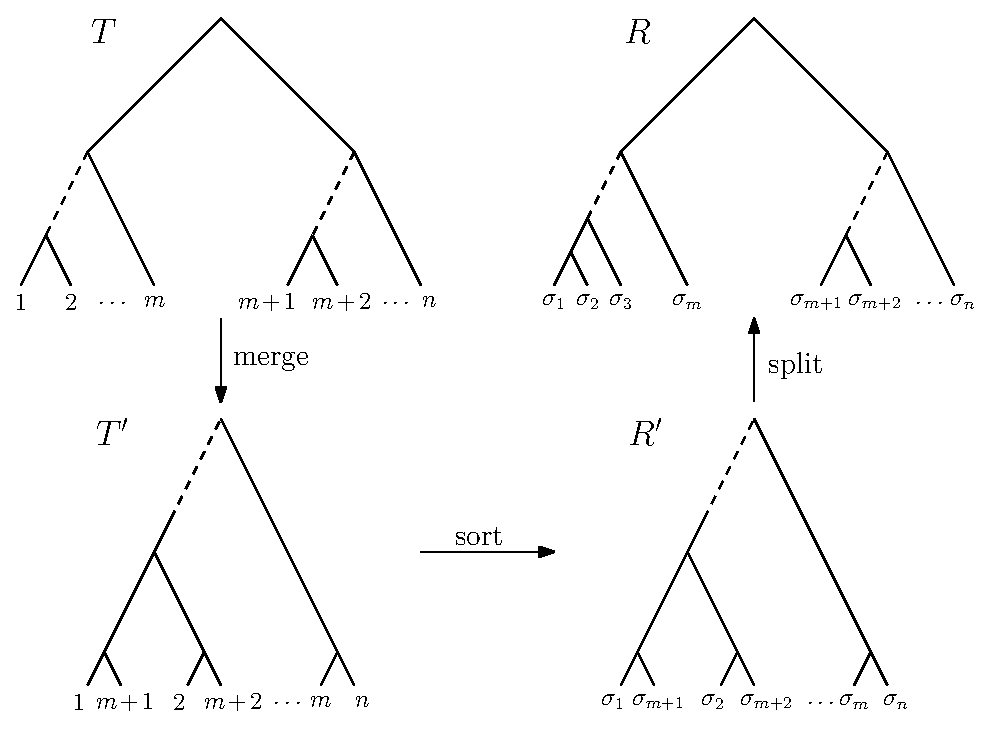
\includegraphics[width=.8\textwidth]{NNI_NP_proof}
\vspace{12pt}
\caption{Example of a shortest path between two trees $T$ and $R$ in $\nni$.
All leaves labelled with dots represent taxa in $\{1, \ldots, n\}$, squares represent taxa in $\{n+1, \ldots, 2n\}$.
In \autocite{Li1996-zw} it is proven that there is such a labelling that ensures that there is no shortest path in $\nni$ where the clusters (dots vs.\ squares) shared between $T$ and $R$ are preserved.
Instead, the depicted path where $n$ cherries are built and then sorted before being resolved is a shortest path}
\label{fig:NNI_NP_proof}
\end{figure}

Since the example given in \autocite{Li1996-zw}, which can be used to prove Theorem~\ref{thm:split_nni} in $\nni$, does not work in $\rnni$, a contrary statement was conjectured in \autocite{Gavryushkin2018-ol}.
For understanding this conjecture it is important to know the connection between edges in a tree and so-called \emph{splits}, which are bipartitions of the taxon set of a tree:
By deleting an edge $e$ of a tree $T$ one receives two graphs with labels in $A$ and $B$, respectively, such that $\{A,B\}$ is a partition of the taxon set of $T$.
Note that each edge induces such a bipartition, often written as $A|B$, and that both edges incident to the root of a tree induce the same partition.
Since these partitions are commonly referred to as splits, the following conjecture was named \emph{Split Theorem} in \autocite{Gavryushkin2018-ol}.

\begin{conjecture}[Split Theorem]
For the $\rnni$ graph the following statement holds:
If a partition of leaves given by an edge is present in two trees $T$ and $R$ then the partition is presented in every tree on every shortest path between $T$ and $R$.
\label{conjecture:split_theorem}
\end{conjecture}

We found a simple counterexample to this conjecture, provided in Figure~\ref{fig:splitthm_counterexample}.

\begin{figure}[H]
\centering
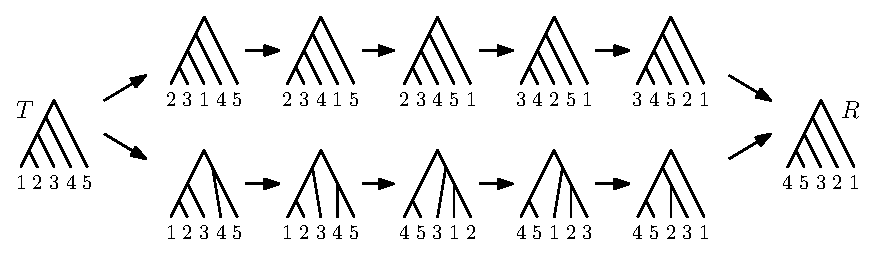
\includegraphics[width=\textwidth]{splitthm_counterexample}
\vspace{12pt}
\caption{The split $123|45$ is present in $T$ and $R$, but the path at the top is a shortest path (computed by $\csort$) where none of the trees contains this split.
On the path at the bottom, which is a shortest path as well, this split is maintained.}
\label{fig:splitthm_counterexample}
\end{figure}

Since the counterexample in Figure~\ref{fig:splitthm_counterexample} shows that the version of the Split Theorem stated in \autocite{Gavryushkin2018-ol} does not hold, we will now claim an alternative to this conjecture, the \emph{Cluster Theorem} (Conjecture~\ref{conjecture:cluster_theorem}).
Within the Cluster Theorem we are considering clusters instead of splits.
This is motivated by the fact that rooted phylogenetic trees can uniquely be represented by sets of clusters \autocite{Steel2016-ye}, but not by sets of splits as they cannot define the position of the root.
Note that trees $T$ and $R$ in Figure~\ref{fig:splitthm_counterexample} induce the same set of splits, but share no cluster.

\begin{conjecture}[Cluster Theorem]
For the $\rnni$ graph the following statement holds:
if two trees $T$ and $R$ contain the same cluster $C$, then $C$ is present as cluster in every tree on every shortest path between $T$ and $R$.
\label{conjecture:cluster_theorem}
\end{conjecture}


For providing further evidence that the Cluster Theorem holds in $\rnni$, we can show computationally that it holds for the $\rnni$ graph on small trees with up to six taxa.
We did this by computing subgraph of $\rnni$ only containing trees that share a cluster and compare distances within this graph with distances in the whole $\rnni$ graph \autocite{}.
\todo{LC: github link}
We computed these graphs according to the algorithm of \autocite{Gavryushkin2018-ol} as discussed in Section~\ref{section:algorithms}.

% \todo{LC: We still need to check 7 taxa.}
% We are doing this in the following way.
% We focus on the subset of trees that induce share a cluster.
% It is sufficient to consider clusters of the shape $\{1, \ldots, m\}$ for $2 \leq m \leq n-1$, because of the symmetry of the space:.
% distances $d(T_1,R_1)$ and $d(T_2,R_2)$ between two pairs of trees $(T_1,R_1)$ and $(T_2,R_2)$ are equal if one can receive $T_2$ from $T_1$ by permuting the taxa the same way as it is necessary for receiving $R_2$ from $R_1$.
% Therefore, we compute for all $m = 2, \ldots, n-1$ exact $\rnni$ distances between all pairs of trees containing the cluster $\{1, \ldots, m\}$, using Dijkstra's algorithm \autocite{Dijkstra1959-ph} on the $\rnni$ graph, which we can compute as explained in Section~\ref{section:alg_RNNI_graph}.
% Additionally, we compute the subgraph of $\rnni$ induced by the subset of trees that include the cluster $\{1, \ldots, m\}$.
% With the Floyd-Warshall algorithm we compute all pairwise distances between the trees in this subgraph and compare them with the distances in $\rnni$.
% With this approach it is possible to show that the Cluster Theorem holds for up to seven taxa.
% \todo{LC: We still need to check 7 taxa.}


% \section{Ideas}
%
% [This section includes some ideas that we could possibly include in the paper]
%
% Using the same argument as in the proof of Lemma~\ref{lemma:distance_delete_taxon} we can establish Proposition~\ref{proposition:lower_bound_distance} that provides a lower bound on the distance between trees.
%
% \begin{proposition}
% If trees $T$ and $R$ and taxon $x$ are such that $|\rank_T(\parent_T(x)) - \rank_R(\parent_R(x))| = \delta$ then $d(T,R) \geq \delta$.
% \label{proposition:lower_bound_distance}
% \end{proposition}
%
%
% The paths computed by $\findpath$ depend on the order of input trees $T$ and $R$:
% $\findpath(T,R)$ does not necessarily produce the reverse path of $\findpath(R,T)$.
% An example can be found in Figure~\ref{fig:findpath_not_symmetric}.
% However, simulations suggest that the lengths of the two paths computed by $\findpath$ for one pair of trees are equal.
%
% \begin{conjecture}
% Let $T$ and $R$ be ranked trees.
% The lengths of paths $\findpath(T,R)$ and $\findpath(R,T)$ are equal.
% \end{conjecture}
%
% \begin{figure}[H]
% \centering
% 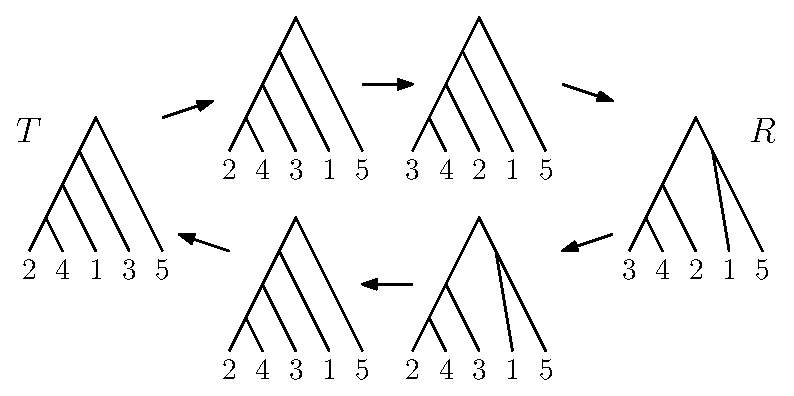
\includegraphics[width=0.7\textwidth]{findpath_not_symmetric}
% \vspace{12pt}
% \caption{Two paths computed by $\findpath$.
% At the top $\findpath(T,R)$, at the bottom $\findpath(R,T)$}
% \label{fig:findpath_not_symmetric}
% \end{figure}
%
% % idea for description of max distance caterpillar trees:
% \begin{lemma}
% Let $T$ and $R$ be caterpillar trees.
% It is $d_c(T,R) = \Delta(\rnni)$ if, and only if, $T$ and $R$ share no induced triplet.
% \todo{define induced triplets}
% \end{lemma}
%
% This Lemma does only hold for caterpillar trees and not for trees with more than one cherry.
% Furthermore, triplets do not represent ranked trees uniquely as they do not contain information about the ranks of internal nodes (but they can uniquely define caterpillar trees as these only have one cherry)
%
% \begin{proof}
% %TODO
% % Insert the proof here
% Fix $T = (\ldots(1,2) \ldots ,n)$, use induction on $n$ and $\csort$ (taxon $n$ must be in cherry of $R$ if distance is max).
% \end{proof}
%
% According to Algorithm~\ref{alg:max_dist_tree}, the number of trees with maximum distance to a given caterpillar tree $T$ is $(n-1)!$.
% The number of caterpillar trees with distance $\Delta(\rnni)$ from a given caterpillar tree is $2^{n-2}$.
%
%
% \subsection{Partition lattice}
%
% % Define Partition Lattice $\Pi_n$ and max chains in that lattice!
%
% \begin{theorem}
% The $\rnni$ graph on $n$ taxa is isomorphic to the graph of maximal chains of the partition lattice $\Pi_n$ where two maximal chains are connected by an edge if and only if they differ by exactly one partition.
% The corresponding metric spaces are isometric.
% \end{theorem}

\section{Discussion}

Within this paper we established some geometric properties of the $\rnni$ graph.
We furthermore pointed out some differences between this graph on ranked trees and the well studied $\nni$ graph on unranked trees.
This is of particular interest for analysing the complexity of computing distances in $\rnni$ as this problem is known to be $\np$-complete in $\nni$.
Our finding that the set of caterpillar trees is convex in $\rnni$ (Theorem~\ref{thm:caterpillar_convex}) suggests that there is a difference in complexity between these two tree spaces.
This leaves hope that computing distances in $\rnni$ is, contrary to this problem in $\nni$, not $\np$-complete.
The question of how hard this problem actually is still remains open and will be subject of further research.

Our work in this paper highlights the importance of algorithms for computing paths in $\rnni$ in order to prove geometric properties such as diameter and radius.
One of the algorithms that has been introduced, $\findpath$, computed exact distances for all pairs of trees on up to six taxa.
For future investigations of the $\rnni$ space this algorithm might be a useful tool.

\printbibliography

\end{document}
